\section{Architecture}
%Refactoring Tool work flow: (add a brief explanation of what does)

%FIXME The Chosen IDE here??


In order to create correct refactoring operations, the refactoring tool uses two sources of
information, the def-use-relations and the AST of the program.
The def-use-relations represent the definition of an identifier and its usage, it is
 visually represented in a form of arrows in DrRacket.

The AST is represented by a list of syntax-objecs which composes the racket program.
%In Racket everything is a syntax-object and therefore accessing the list
%of syntax-objects has all the information that a normal AST provides. %FIXME incorrect


\begin{figure}
\centering
\tikzstyle{startstop} = [rectangle,  minimum width=2cm, minimum height=1cm,text centered, draw=black, fill=red!30] %start
\tikzstyle{process} = [rectangle,  minimum width=2cm, minimum height=1cm, text centered, draw=black, fill=orange!30] %process
\tikzstyle{process2} = [rectangle,  minimum width=2cm, minimum height=1cm, text centered, draw=black, fill=blue!30]
\tikzstyle{process3} = [rectangle,  minimum width=2cm, minimum height=1cm, text centered, draw=black, fill=blue!30]
\tikzstyle{process4} = [rectangle,  minimum width=3cm, minimum height=2.5cm, draw=black, fill=blue!30]
\tikzstyle{arrow} = [thick,->,>=stealth]
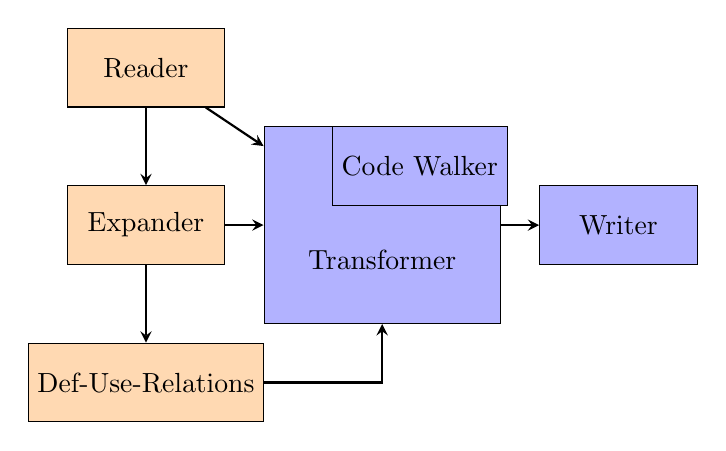
\begin{tikzpicture}[node distance=2cm]
\node (pro1) [process] {Reader};
\node (pro2) [process, below of=pro1] {Expander};
\node (pro3) [process, below of=pro2] {Def-Use-Relations};
\node (pro5) [process4, right of=pro2, xshift=1cm, align=left] { \\[2em] Transformer};
\node (pro4) [process3, xshift=-1.03cm, yshift=0.75cm] at (pro5.east) {Code
 Walker};
\node (pro6) [process2, right of=pro5, xshift=1cm] {Writer};
\draw [arrow] (pro1) -- (pro2);
\draw [arrow] (pro2) -- (pro3);
\draw [arrow] (pro1) -- (pro5);
\draw [arrow] (pro2) -- (pro5);
\draw [arrow] (pro3) -| (pro5);
%\draw [arrow] (pro4) -- (pro5);
%\draw [arrow] (pro5) -- node[anchor=east] {use} (pro4);
\draw [arrow] (pro5) -- (pro6);
\end{tikzpicture}
\caption{Main modules and information flow between modules. Unlabeled arrows represent information
flow between modules.}
\label{flow-chart}
\end{figure}

Figure~\ref{flow-chart} summarizes the work flow of the refactoring tool where
the Reader produces the non expanded AST of the program while the Expander expands the
AST produced by the Reader.
In order to produce the def-use-Relations it is necessary to use the expanded AST produced by the
Expander because it has the correct dependency information.
The Transformer uses the Code Walker to parse the ASTs and the information of the Def-Use-Relations
to correctly perform the refactoring operations.
 Then it goes to the Writing module to produce the output in DrRacket's definitions area.


\subsection{Syntax Expressions}
%intro and explain the importance of the S-Exp
The syntax-object list represent the AST, which provides information about
the structure of the program.
The syntax-object list is already being produced and used by the Racket language and
in DrRacket in order to provide error information to the user.
DrRacket already provides functions which computes the program's syntax-object list and uses some of those
functions in the Background Check Syntax and in the Check Syntax button callback.


\subsubsection{Syntax Expression tree forms}
DrRacket provides functions to compute the syntax-object list in two different formats.
One format is the expanded program, which computes the program with all the macros expanded.
The other format is the non-expanded program and computes the program with the macros
unexpanded.

The expanded program has the macros expanded and the identifier information correctly
computed.
However, it is harder to extract the relevant information when compared with the
non expanded program.


For example, the following program is represented in the expanded program,
and in the non expanded program.

\begin{lstlisting}[basicstyle=\ttfamily, caption=Original Code]
(and alpha beta)
\end{lstlisting}

\begin{lstlisting}[basicstyle=\ttfamily, caption=Expanded program]
#<syntax:2:0
 (#%app call-with-values
 (lambda ()
    (if alpha beta (quote #f)))
  print-values)>
\end{lstlisting}

\begin{lstlisting}[basicstyle=\ttfamily, caption=Non-expanded program]
#<syntax:2:0 (and alpha beta)>
\end{lstlisting}


The expanded program transforms the {\tt and}, {\tt or}, {\tt when}, and {\tt unless} forms into
{\tt if}s which makes refactoring operations harder to implement.

Racket adds internal representation information to the expanded-program which for
most refactoring operations is not necessary.
In addition, the expanded program has a format that is likely to change
in the future.
Racket is an evolving language and the expanded form is a low level and internal
form of representation of the program.
However, the expanded program has important information regarding the binding
information that is not available in the non-expanded form and is rather useful
to detect if two identifiers refer to the same binding.
Additionally we do not consider macros as part of a code that could be refactored,
 since the refactoring tool is targeted at unexperienced programmers macros
will not be used often and therefore it is not considered part of the scope of
this refactoring tool capabilities.

Therefore it is desirable to use the non expanded form for the refactoring %all things considered
operations whenever possible and use the expanded form only for the necessary
operations.
Nevertheless, if we intended to create a tool that gives support to refactoring macros
we would need to use the expanded program.
However, there are no guarantees that would be enough to ensure the correctness of
such refactoring operations due to the reflection capabilities of Racket.


\subsection{Def-Use-Relations}
Def-Use-Relations holds an important information in order to produce correct refactoring operations.
They can be used to check whether or not there will be a duplicated name
or even to compute the arguments of a function to be extracted.

DrRacket already uses the def-use-relations in the system and they are visually  %TODO they are or it is?
represented by arrows in the GUI.
The def-use-relations is computed by the online-compiler that runs in the background.
However, it is only computed when a program is syntactically correct.

\subsection{Code-walker}
The code-walker is used to parse the syntax tree represented by a syntax elements
that is a list of syntax-object in Racket.
A syntax-object can contain either a symbol, a syntax-pair, a datum (number, boolean or string),
or an empty list.
While a syntax-pair is a pair containing a syntax object as it first element and
either a syntax pair, a syntax element or an empty list as the second argument.
Each syntax-object has information about the line where they are defined and this
information is to search for the correct elements.


Most of the time using the code-walker we are searching for a specific syntax element
and location information contained in the syntax-object  is used to skip the syntax
 blocks that are before the syntax element wanted in the first place.

The Code-walker is a core part of the refactoring tool ensuring that the selected
syntax is correctly fed to the refactoring operations. %actually?


\subsection{Pretty-printer}
Producing correct output is an important part of the refactoring tool.
It is necessary to be careful to produce indented code and we decided to use a pretty-printer
that is already incorporated in the language.
However, this pretty-printer does not follow the convention in the {\tt cond} clauses
should be surrounded by {\tt [ ] } parenthesis. This is not considered a problem because
Racket supports both representations.
One possible solution is to use a different pretty-printer in
order to keep the language convention.


\subsection{Comments preservation}
Preserving the comment information after a refactoring transformation is an important task
of the refactoring tool. If the comment in determined place of the program
changes its location affecting another structure it could confuse the programmer.
However, comment preservation is not implemented yet, making it a limitation of
this prototype.

One possible solution is to modify the syntax reader and add a comment node to the
AST.
While the new node will not be used during refactoring transformations it is used
during the output part of the refactoring operation preserving the comment with
the correct syntax expression.


\subsection{Syntax-Parse}

The Syntax-Parse function provided by Racket is rather useful for the refactoring
operations regarding mainly syntax information.
It provides a wide range of options to help matching the correct syntax with  %fine tunning
backtracking making it possible to have several rules to be matched
in the same syntax parser, which helps to create more sophisticated rules.

\section{Refactoring operations}
%TODO do introduction
In this section we explain some of the  more relevant refactoring operations and
some limitations of the refactoring tool.

\subsection{Semantic problems}
There are some known semantic problems that might occur after doing a refactoring
operation.
One of them occurs in the refactoring operation that removes redundant {\tt and}s
in numeric comparisons, since Racket supports more than two arguments.
\begin{lstlisting}[basicstyle=\ttfamily, caption=And example]
  (and (< 1 (foo 2)) (< (foo 2) 3))
  (define (foo arg)
    (displayln "foo")
    arg)
\end{lstlisting}
The refactoring transforms the code into this:
\begin{lstlisting}[basicstyle=\ttfamily, caption=Refactored code]
  (< 1 (foo 2) 3)
\end{lstlisting}


Instead of applying the side effect that is displaying the the string "foo"
 twice it will only display it once. Therefore changing the meaning of the program.

We still kept this refactoring operation because in the vast majority
of the cases this refactoring operation do not change the semantic of the program.
Furthermore, the possible solution would limit excessively this refactoring operation.  %enormously
Considering Racket's reflection capabilities we would only apply this refactoring operation
safely when the arguments of the {\tt <} expressions, in this case the numbers 1, 2, 3, and the function {\tt foo}
 were datums (number, boolean or string).


Another example of a semantic problem occurs when refactoring the following {\tt if}
expression.
\begin{lstlisting}[basicstyle=\ttfamily, caption=Code sample]
(if ?x
    (begin ?y ...)
    #f)
\end{lstlisting}
There are two different refactoring transformations possible:
\begin{lstlisting}[basicstyle=\ttfamily, caption=Refactoring option 1]
(when ?x
      ?y ...)
\end{lstlisting}

\begin{lstlisting}[basicstyle=\ttfamily, caption=Refactoring option 2]
(and ?x (begin ?y ...))
\end{lstlisting}

The first refactoring option changes the meaning of the program, because if the
test expression, in this case {\tt ?x}, is false the result of the {\tt when} expression is {\tt \#<void>}.
However, the programmer may still want to choose the first refactoring option if
the return value when the {\tt if} is false is not important creating a dilemma,
there are two possible refactoring operations applicable.
For example, if a programmer is creating a predicate may
choose the {\tt and} version, whereas if the programmer is using another control structure
and do not care for the result of the expression may prefer the {\tt when} version.

\subsection{Extract Function}
Extract function is an important refactoring operation that every refactoring tool
should have.
In order to extract a function it is necessary to compute the arguments needed
to the correct use of the function.
While giving the name to a function seams quite straightforward it is necessary to
check for name duplication in order to produce a correct refactoring. e.g. Having
two identifiers with the same name and in the same scope produces an incorrect program
and therefore modifying the meaning of the program.
Lastly, computing the function body and replacing it by the call should be straightforward.

However, it raises the problem where should the function be extracted to. A function can not
be defined in an expression, (e.g inside a {\tt let}) but it could be defined in the top-level
or in any other level that is accessible from the current level.

e.g: When extracting the {\tt (+ 1 2)} to a function where should it be defined?
Top-level, Level-0, level-1, or in the current level, the level-2?
\begin{lstlisting}[basicstyle=\ttfamily, caption=Extract function levels]
;;top-level
(define (level-0)
  (define (level-1)
    (define (level-2)
      (+ 1 2))
    (level-2))
  (level-1))
\end{lstlisting}

The fact is that is extremely difficult to know the answer to this question because
it depends on what the user is doing and the user interpretation.
Accordingly we decided that the best solution is to let the user decide where
the user wants the function defined.


\subsubsection{Computing the arguments}

In order to compute the arguments we have to know in which scope the variables are being defined, in other words,
if the variables are defined inside or outside the extracted function. %FIXME it is weird
The variables defined outside the function to be extracted are the candidates to be the arguments %FIXME IMPROVE
of that function.
However, imported variables, whether from the language base or from other libraries
does not have to be passed as arguments, to solve this we considered two possible solutions:

  -Def-use-relations + Text information

  -Def-use-relations + AST

The first approach is simpler to implement and more direct than the second one.
However, it is less tolerant to future changes and to errors.
The second one combines the def-use-relations information with the syntax information to
check whether it is imported from the language or from other library.

We choose the second approach in order to provide a more stable solution to compute
 correctly the arguments of the new function.

\subsection{Let to Define Function} %implemented is it worth it?
%Refactoring Let to Defines Usefulness Vs implementation difficulty

%there are several let forms, we want to focus on let* let and named let.
A {\tt let} expression with a function has similarities with a function, which may led
to mistakenly choose the {\tt let} expression instead of a function and vice-versa.
Therefore we decided to provide a refactoring operation that would make that transition simpler.

There are several let forms, but we want to focus in the ones more similar to
a function, namely the {\tt let} and the {\tt named let}.

The {\tt let} and the {\tt named let} can be directly mapped to a function, however, the {\tt named let}
 can be directly mapped to a named function, the {\tt define} keyword, whereas the {\tt let} can only be directly mapped
to an anonymous function.
However, we did not consider the transformation of a {\tt let} to an anonymous function, {\tt lambda},
making the code simpler and therefore it was not implemented yet.\\


A refactoring operation that transform a {\tt named let} into a {\tt define} function,
 could have syntax problems because a {\tt let} form can be used in expressions, but the {\tt define} can not.
In the vast majority of cases this refactoring is correct, but when a {\tt let} is used in an expression
it is not correct and it changes the meaning of the program, transforming a correct
program in a incorrect one.
e.g.
\begin{lstlisting}[basicstyle=\ttfamily, caption=Let in an expression]
(and (let xpto ((a 1)) (< a 2)) (< b c))
\end{lstlisting}
Modifying this {\tt named let} into a define would raise a syntax error because a
define could not be used in an expression context.
This could be solved by using the local keyword that is an expression like
the let form.
However, the {\tt local} keyword is not used very often and might confuse the users.
This reason made us keep the refactoring operation without the local keyword that works for
most of the cases.


\subsection{Wide-Scope Replacement} %is this a feature or a refactoring?
The Wide-Scope replacement extends the functionality of the extract function refactoring
by replacing the duplicated of the extracted code with a function call to the new function.


The Wide-Scope replacement refactoring operation searches for the code that is duplicated of the extracted
function and then replaces it for the call of the
extracted function and it is divided in two steps: %FIXME Improve

- Detect duplicated code

- Replace the duplicated code

Replacing the duplicated code is the easy part, however the tool might has to compute %have?
the arguments for the duplicated code itself.

\subsubsection{Detecting duplicated code}
Correctly detect duplicated code is a key part for the correctness of this refactoring.
Even the simplest form of duplicated code detection, when it only detects duplicated code
when the code is exactly equal, may have some problems regarding the binding information.
For example, if the duplicated code is inside a {\tt let} that changes some bindings that must
be taken into consideration.
In order to solve the binding problem we can use functions already provided in Racket.
However, that does not work if we use the program in the not expanded
form to do the binding comparisons because there is not enough information for those bindings to work. %FIXME improve :(

%[TODO Recently racket changed binding expansion and it brought interesting improvements to racket and that might be useful for this, read paper before]

Therefore, in order to compute the correct bindings, it is necessary to use the expanded form
of the program.

The naive solution is to use the expanded program to detect the duplicated
 code and then use this information to do the replacing of the duplicated code.
However, when expanding the program Racket adds necessary internal information to
run the program itself that are not visible for the user.
While this does not change the detecting of the duplicated code, it adds unnecessary information
that would have to be removed. %FIXME
In order to solve this problem in a simple way we can use the expanded code to detect
the correctly duplicated code and use the non expand program
to compute which code will be replaced.

However, this detection is a quadratic algorithm which might
have some performance problems for bigger programs.

%Detecting duplicated code can be added to the automatic detection of possible refactoring operations to be applied. %FIXME is this already done?
%Notifying the users of a possible extract function operation if there is duplicated code is a rather
%useful because sometimes it might be difficulty for the user to remember if a
%piece of code is duplicated or not.

\subsection{Refactoring Python}
Python is being promoted as a good replacement for Scheme and Racket in science introductory courses.
It is an high-level, dynamically typed programming language it supports the functional, imperative and object
oriented paradigms.
Using the capabilities offered by Racket and DrRacket with an implementation of Python for Racket\cite{ramos2014implementation} \cite{ramos2014reaching}
we also can also have refactoring operations in Python.
%focus in the functional paradigm of Python
Using Racket's syntax-objects to represent Python like a meta-language like it was used in FAMIX\cite{tichelaar2000meta}.
It is possible use the same structure to parse and analyze the code used for the refactoring operations in Racket.

However, there are some limitations regarding the refactoring operations in Python.
Since Python is a statement base language instead of expression base, it raises
some problems regarding the possibility of some refactoring operations.
